%-------------------------------------------------------------------------------
\section{Problem}\label{s:problem}
%-------------------------------------------------------------------------------

In order to understand the poor isolation of the LC workload in our experiment,
we analyze perf traces of the scheduling decisions.

\subsection{The problem}

\begin{figure}[t]
    \centering
    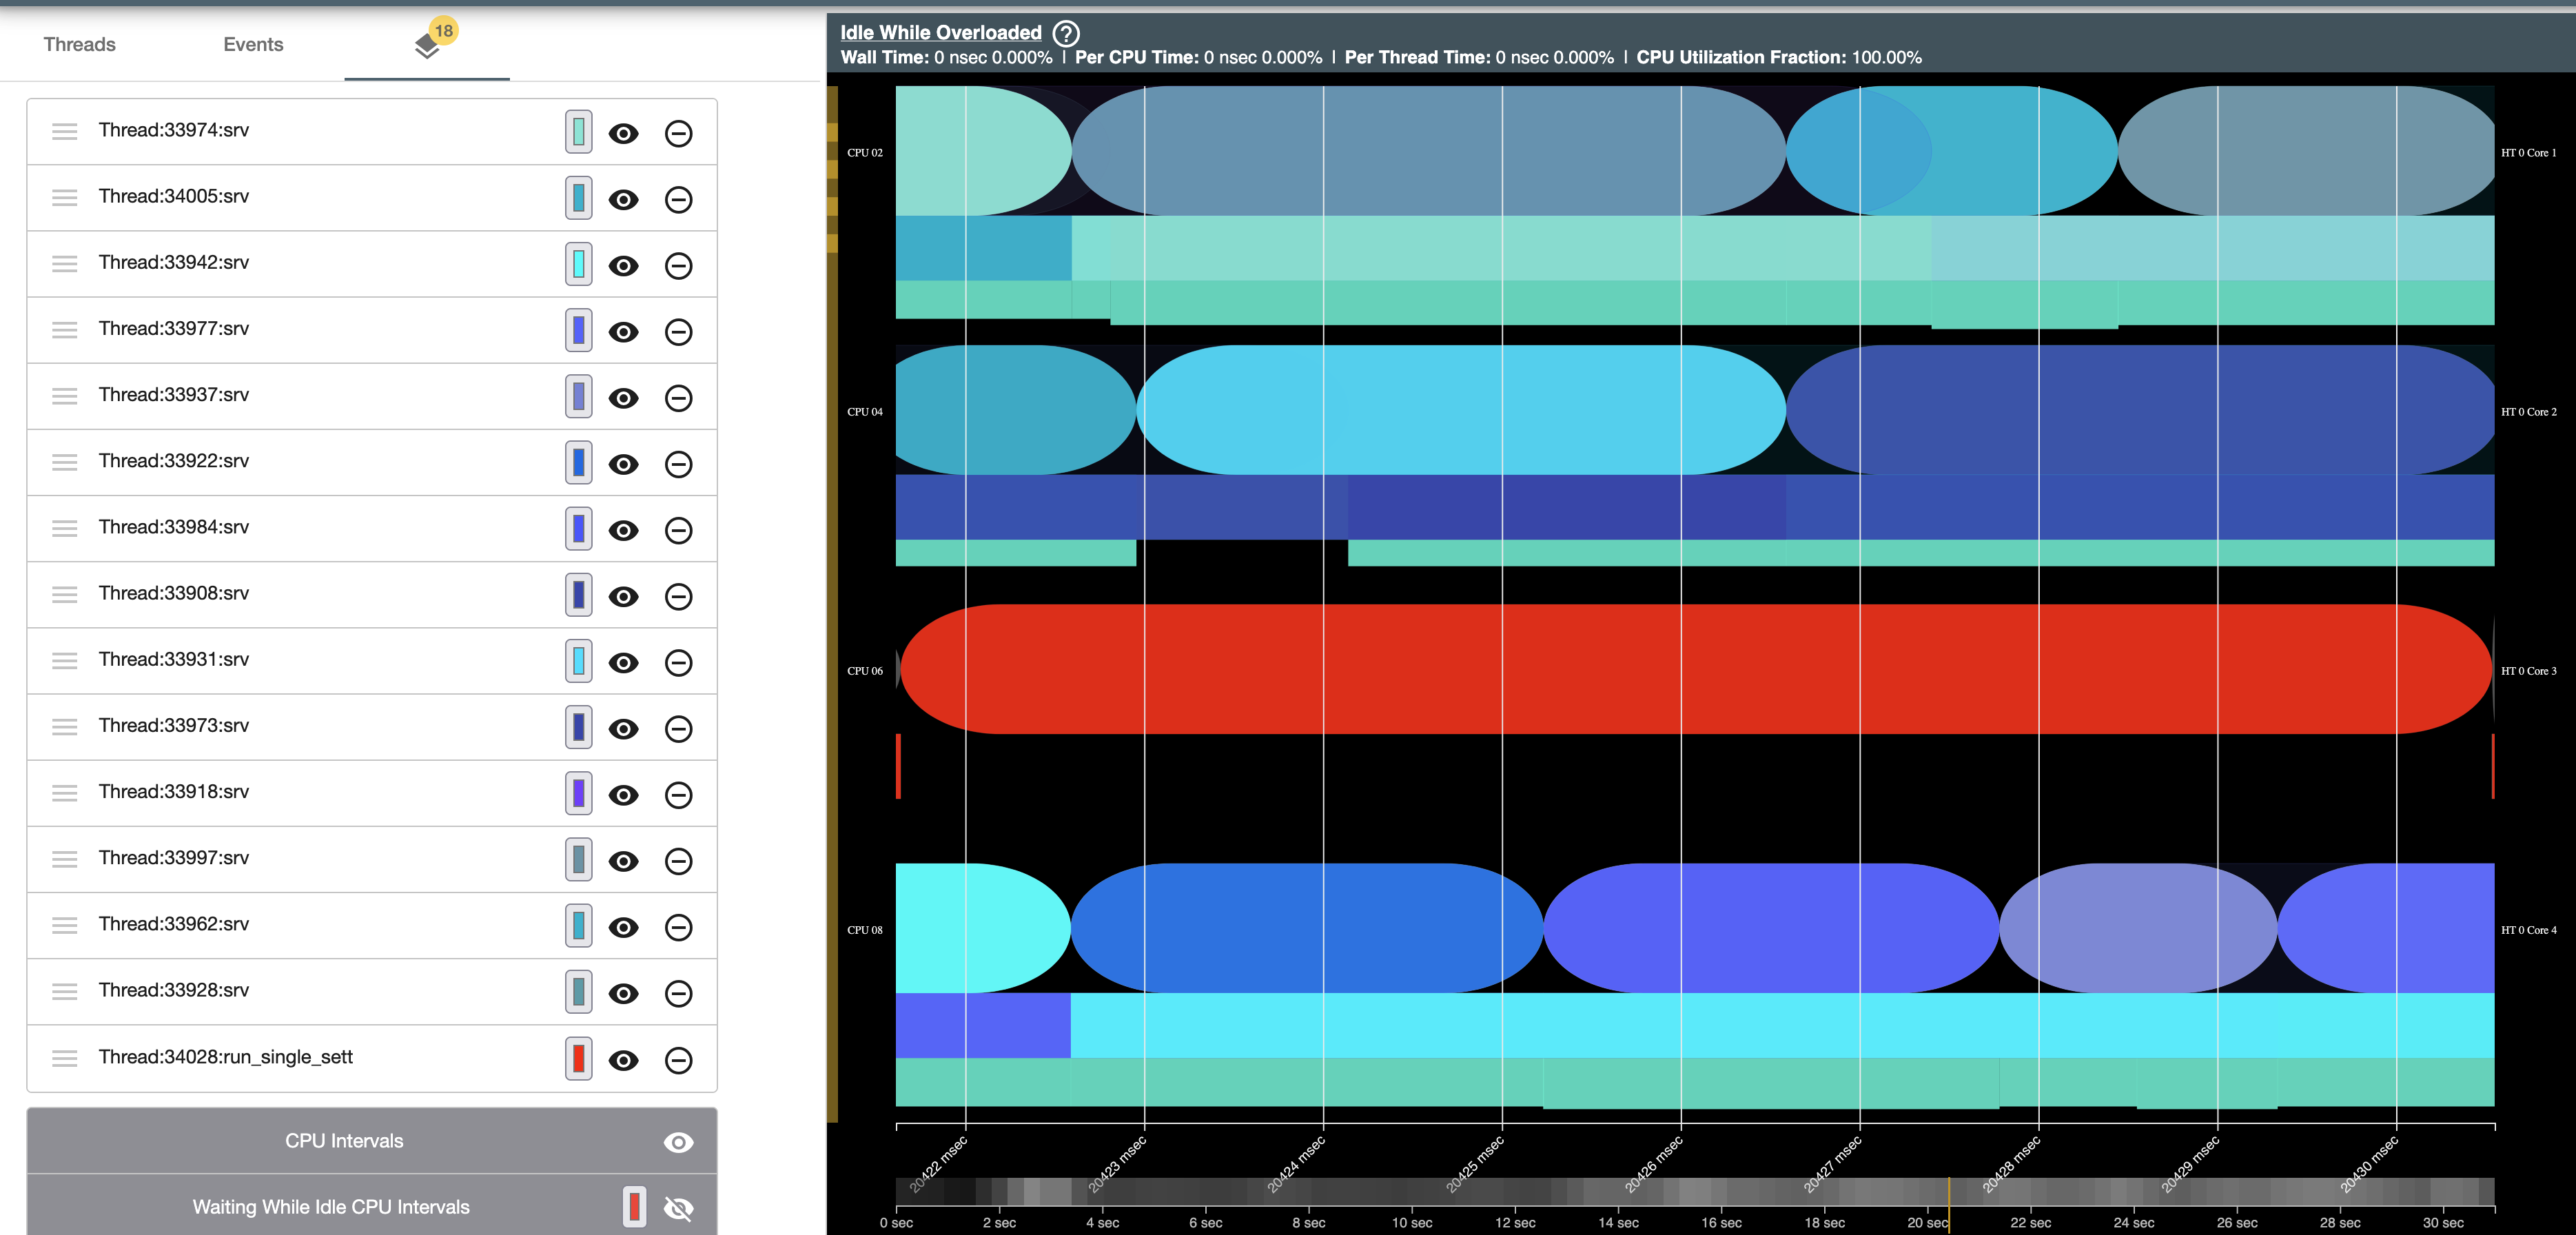
\includegraphics[width=\columnwidth]{graphs/schedviz.png}
    \caption{Each thread is a different color. Circles represent which
    thread is running on that core, while rectangles underneath show waiting but
    runnable threads. Core numbers are 2,4,6,8 because this was run on a NUMA
    node so those are the cores that are closest to each other
    }\label{fig:schedviz}
\end{figure}

The failure mode we observe when looking at these traces is that \textit{one
core is running a BE process, while an LC process is waiting on another}. We
visualize the trace using schedviz~\cite{TODO}; a 10ms outtake of the resulting
image is show in \autoref{fig:schedviz}. The process running on each core is
shown as a an oval, and queued processes are shown as rectangles below. The root
of the undesirable behavior is clear: on core 6, the red process that is running
the whole time is a BE process, whereas LC threads, shown in varying shades of
blue, are queued on the other cores.

The reason this happens is that Linux maintains a separate runqueue on each
core, in order to avoid the synchronization overheads of accessing global state
for every scheduling decision. Within each runqueue, Linux does a pretty good
job of maintaining the correct ratio of received cputime; but it does not
enforce the weight ratios across cores. This leads to the above failure mode,
where one core has no runnable high weight processes and thus runs a low weight
one, whereas another core has queued high weight processes. This problem goes
away when there are no BE processes, because cores try to steal work before
going idle.

\subsection{It's the interface, not the implementation}

The root of the problem goes deeper than just a poor implementation: in a
setting of per-core runqueues where synchronization is expensive, a weight-based
interface is at odds with machine-wide policy enforcement.

Changing the implementation to correctly enforce the current interface is an
unappealing proposition for two main reasons: (1) small weights are still
weights, and (2) enforcing a split across cores requires more synchronization
than enforcing a strict priority.

Although low weights run infrequently, they still get a fair share, and in doing
so impact the latency of the higher weight (LC) processes. A large number of BE
workloads each with a small weight could add up to represent a significant
amount of weight in the system, now contending directly with the LC workload.
Weights also interact with Linux's 4ms scheduling tick granularity in an
unfortunate way: when it is a low-weight processes time to run, it will
likely be scheduled for a full tick. It is common for microservices to have SLAs
in the order of 10ms or even less, where a gap of 4ms will have a significant
impact on response latency. Compounded with a large number of BE workloads, this
can lead to significant overheads even in a world where weights are correctly
enforced across cores.

Additionally, in order to strictly enforce a weight split globally, the
scheduler would need to synchronize at every scheduling decision: calculating
whether a given process is owed time globally requires knowing the total weight
across all cores as well as the sum of time that all the processes in the group
have gotten. Optimizations could reduce the frequency of synchronication, but at
a cost to correctness: Linux load balances periodically, but this does not
preclude the observed problem from happening. That being said, migration already
does improve the performance: in \autoref{fig:schedviz}, we can see that the
experiment uses cores 2,4,6, and 8, rather than the potentially more obvious
0-5. This is because the machine we ran this experiment on had NUMA nodes, and
the results were much worse when using cores 0-5, because migration is more
expensive and thus rarer across NUMA nodes.




